%% Type de document et encodage de la police
\documentclass[a4paper]{article}
\usepackage[utf8x]{inputenc}
\usepackage[T1]{fontenc}
\usepackage[colorlinks=true, allcolors=black]{hyperref}
% \usepackage[french]{babel}

%% Initialise la taille des pages et des marges
\usepackage[a4paper, top=3cm, bottom=3cm, left=2cm, right=2cm, marginparwidth=2cm]{geometry}

%% Packs utiles
\usepackage{amsmath}
\usepackage{graphicx}
\usepackage[shortlabels]{enumitem}

%% Commandes perso
\renewcommand{\arraystretch}{1.2} %% row 20% longer
\renewcommand{\contentsname}{Table des matières}

%% Pour les exemples
\usepackage{mdframed}
\newmdenv[topline=false, bottomline=false, rightline=false, skipabove=\topsep, skipbelow=\topsep]{example}

%% Pour les diagrammes
\usepackage{tikz}
\tikzstyle{incolore} = [rectangle, rounded corners, draw=black, minimum height=1cm, minimum width=3cm, text width=3cm, text centered]


\title{OS Propriétaire Labo -- Notes}
\author{Grégoire Roumache}
\date{Septembre 2020}

\begin{document}

\maketitle

\tableofcontents















\section{Labo 1 -- Active Directory}





% \begin{enumerate}

% \item Installer windows 10 \& 2 windows server 2019, les placer dans un réseau privé/interne.

% \item Configurer une 1ère machine windows server 2019:
% \begin{enumerate}
%     \item utiliser \texttt{sysprep} (abréviation de \textit{system preparation}, à utiliser si vous avez cloné la windows server)
%     \item changer le nom système de la machine en \textit{DC1}
%     \item ajouter un compte local
%     \begin{itemize}
%         \item username = User1
%         \item password = PasswordDC1
%     \end{itemize}
%     \item activer la règle de parefeu pour ping
%     \item modifier la config réseau
%     \begin{itemize}
%         \item ip = 192.168.0.2
%         \item netmask = 255.255.255.0 (/24)
%         \item dns = 192.168.0.130
%     \end{itemize}
%     \item installer l'active directory
%     \item ajouter un compte nommé \textit{Pamela} dans l'active directory
%     \item ajouter une unité d'organisation dans l'active directory \textit{Staff}
%     \item déplacer le compte \textit{Pamela} dans l'unité d'organisation \textit{Staff}
% \end{enumerate}

% \item Configurer une 2ème machine windows server 2019:
% \begin{enumerate}
%     \item changer le nom système de la machine en \textit{MS1}
%     \item ajouter un compte local
%     \begin{itemize}
%         \item username = User1
%         \item password = PasswordMS1
%     \end{itemize}
%     \item activer la règle de parefeu pour ping
%     \item modifier la config réseau
%     \begin{itemize}
%         \item ip = 192.168.0.130
%         \item netmask = 255.255.255.0 (/24)
%         \item dns = 192.168.0.130
%     \end{itemize}
%     \item intégrer la machine à l'active directory
% \end{enumerate}

% \item Configurer la windows 10:
% \begin{enumerate}
%     \item changer le nom système de la machine en \textit{PC1}
%     \item ajouter un compte local
%     \begin{itemize}
%         \item username = User1
%         \item password = PasswordPC1
%     \end{itemize}
%     \item activer la règle de parefeu pour ping
%     \item modifier la config réseau
%     \begin{itemize}
%         \item ip = 192.168.0.65
%         \item netmask = 255.255.255.0 (/24)
%         \item dns = 192.168.0.130
%     \end{itemize}
%     \item intégrer la machine à l'active directory
% \end{enumerate}

% \item Tester la configuration:
% \begin{enumerate}
%     \item sur chaque machine, ping les adresses suivantes:
%     \begin{itemize}
%         \item 192.168.0.65
%         \item 192.168.0.130
%         \item 192.168.0.2
%     \end{itemize}
%     \item se connecter avec le compte active directory \textit{Pamela} sur toutes les machines
%     \item sur le compte \textit{Pamela}, taper la commande: \texttt{gpresult /R}
%     \item se connecter avec le compte active directory \textit{administrator} sur toutes les machines
%     \item se connecter avec les comptes locaux sur toutes les machines
% \end{enumerate}

% \end{enumerate}





\begin{center}
    \begin{tabular}{|p{5cm}|p{5cm}|p{5cm}|} \hline

        %% sur les 3 colonnes (pas de barre de séparation)
        \multicolumn{3}{|p{15cm}|}{
            \begin{enumerate}[(a)]
                \item installer 2 windows server et 1 windows 10
            \end{enumerate}
        }

        \\ \hline

        \begin{center} \textbf{Windows Server n°1} \end{center} &
        \begin{center} \textbf{Windows Server n°2} \end{center} &
        \begin{center} \textbf{Windows 10} \end{center} \\ \hline

        \begin{enumerate} \setcounter{enumi}{-1}
            \item utiliser \texttt{sysprep}
        \end{enumerate}

        && \\ \hline

        \begin{enumerate}
            \item nom système = DC1
            \item ++ User1, PasswordDC1
            \item règle parefeu pour ping
            \item config réseau
            \begin{itemize}
                \item ip = 192.168.0.2/24
                \item dns = 192.168.0.130
            \end{itemize}
            \item installer l'active directory
            \item ++ \textit{Pamela} dans l’AD
            \item ++ unité d’organi. \textit{Staff}
            \item placer \textit{Pamela} dans \textit{Staff}
        \end{enumerate}
        &
        \begin{enumerate}
            \item nom système = MS1
            \item ++ User1, PasswordMS1
            \item règle parefeu pour ping
            \item config réseau
            \begin{itemize}
                \item ip = 192.168.0.130/24
                \item dns = 192.168.0.130
            \end{itemize}
            \item intégrer la machine à l’AD
        \end{enumerate}
        &
        \begin{enumerate}
            \item nom système = PC1
            \item ++ User1, PasswordPC1
            \item règle parefeu pour ping
            \item config réseau:
            \begin{itemize}
                \item ip = 192.168.0.65/24
                \item dns = 192.168.0.130
            \end{itemize}
            \item intégrer la machine à l’AD
        \end{enumerate}

        \\ \hline

        %% sur les 3 colonnes (pas de barre de séparation)
        \multicolumn{3}{|p{15cm}|}{
            \begin{enumerate}[(a)]
                \item tester le ping
                \item se connecter avec \textit{Pamela}, \textit{administrator}, \textit{User1}
            \end{enumerate}
        }

        \\ \hline

    \end{tabular}
\end{center}















\section{Labo 2 -- Gestion des Group Policy Object (GPO)}





\begin{center}
    \begin{tabular}{|p{7.5cm}|p{7.5cm}|} \hline

        \begin{center} \textbf{Windows Server n°1} \end{center} &
        \begin{center} \textbf{Windows Server n°2} \end{center} \\ \hline

        \multicolumn{2}{|p{15cm}|}{
            \begin{enumerate}[(a)]
                \item désactiver les règles de trafic entrant de l'icmp dans le firewall
                \item changer le statut de la section \textit{domain networks} du firewall en \textit{connected}
            \end{enumerate}
        }

        \\ \hline

        \begin{enumerate}
            \item ++ stratégie GPO \textit{log non locally} pour \textit{Pamela} sur DC
            \item ++ unité d'organisation \textit{batimentA} + \textit{batimentA/\{Floor1,Floor2, Servers\}} + \textit{Femmes}
            \item placer MS1 dans \textit{Servers}, \textit{PC1} dans \textit{Floor2}, \textit{Pamela} dans \textit{Femmes}
            \item ++ stratégie GPO \textit{firewall autoriser icmp entrant} sur \textit{Servers}
            \item ++ stratégie GPO \textit{firewall interdire icmp entrant} sur \textit{Default Domain Policy}
            \item ++ stratégie GPO \textit{firewall autoriser icmp entrant} sur \textit{Floor2}
            \item ++ redirecteurs conditionnels (dns), monsite1.local + monsite2.local = 192.168.0.130
            \item ++ préférence GPO \textit{page d'accueil IE = monsite1} sur \textit{Femmes}
        \end{enumerate}
        &
        \begin{enumerate}
            \item installer les rôles DNS et Web
            \item ++ 2 zones primaires, dedans: enregistrement A = \textit{www}
            \item ++ \textit{monsite1} \& \textit{monsite2} (config IIS)
            \item se connecter avec l'administrateur de l'AD
            \item installer le rôle DHCP, l'activer pour l'AD
        \end{enumerate}

        \\ \hline

        \multicolumn{2}{|p{15cm}|}{
            \begin{enumerate}[(a)]
                \item forcer l'adoption immédiate des GPO
                \item vérifier les GPO dans le \textit{Group Policy Management}
                \item aller sur \textit{www.monsite1.local} et \textit{www.monsite2.local}
                \item se connecter en \textit{Pamela} et ouvrir internet explorer
                \item tester le ping
            \end{enumerate}
        }

        \\ \hline

    \end{tabular}
\end{center}















\section{Labo 3 -- Mise en place du NAT}





\begin{center}
    \begin{tabular}{|p{7.5cm}|p{7.5cm}|} \hline

        \begin{center} \textbf{Windows Server n°1} \end{center} &
        \begin{center} \textbf{Windows Server n°2} \end{center} \\ \hline

        \begin{enumerate}
            \item ++ disque de 50 GB (+ initialiser le disque)
            \item ++ nouveau volume \& share de type SMB
            \item ++ stratégie GPO, réduire l'intervalle d'actualisation des GPO
            \item ++ stratégie GPO, interdire notepad aux utilisateurs
            \item ++ unité d'organisation \textit{no\_notepad\_OU}, y placer l'UO \textit{no\_notepad\_OU\_child}
            \item ++  utilisateurs, dans les UO correspondantes: \textit{no\_notepad}, \textit{no\_notepad\_child}
            \item ++ GPO \textit{lock\_taskbar}, enforcer la GPO
            \item bloquer l'héritage pour \textit{no\_notepad\_OU}
            \item ++ filtre WMI: mémoire libre $ > $ 2Go
            \item ++ GPO déployement d'application, ex: chrome (.msi)
            \item ++ modèle d'administration de l'application (.adm)
            \item ++ GPO page d'accueil du navigateur
        \end{enumerate}
        &
        \begin{enumerate}
            \item ++ carte réseau en nat
            \item la configurer en dhcp, dns = 192.168.0.2
            \item ++ rôle \textit{remote access} (nat)
        \end{enumerate}

        \\ \hline
        
        \multicolumn{2}{|p{15cm}|}{
            \begin{enumerate}[(a)]
                \item tester le ping vers internet
                \item accéder au \textit{share} dans l'explorateur de fichiers
                \item tester l'accès à notepad pour les différents utilisateurs
                \item vérifier si la barre des tâches est vérouillée pour les différents utilisateurs
                \item réduire la ram, rebooter la machine et vérifier que l'application n'est pas déployée
                \item augmenter la ram, rebooter la machine et vérifier que l'application est bien installée
                \item tester la page d'accueil du navigateur
            \end{enumerate}
        }

        \\ \hline

    \end{tabular}
\end{center}

\textbf{Exercice supplémentaire}:
\begin{itemize}
    \item les utilisateurs des groupes \textit{firefox\_group} et \textit{chrome\_group} ont leurs navigateurs respectifs installés
    \item les utilisateurs des groupes \textit{monsite1} et \textit{monsite2} ont leurs page d'accueil respectives mises en place
\end{itemize}















\section{Labo 4 -- Gestion des profils et des environnements}





\begin{center}
    \begin{tabular}{|p{7.5cm}|p{7.5cm}|} \hline
        \multicolumn{2}{|p{15cm}|}{ \begin{center} \textbf{Windows 10} \end{center} }

        \\ \hline

        \multicolumn{2}{|p{15cm}|}{
            \begin{enumerate}
                \item ++ répertoires \textit{C:$\backslash$programmes$\backslash$allowed}, et \textit{C:$\backslash$programmes$\backslash$denied}
                \item copier dans ces répertoires \textit{C:$\backslash$Windows$\backslash$System32$\backslash$calc.exe}
                \item copier \textit{C:$\backslash$Windows$\backslash$System32$\backslash$mspaint.exe} sur le share
            \end{enumerate}
        }

        \\ \hline

        \begin{center} \textbf{Windows Server n°1} \end{center} &
        \begin{center} \textbf{Windows Server n°2} \end{center} \\ \hline

        \begin{enumerate}
            \item ++ OU \textit{roaming\_OU}
            \item ++ utilisateur itinérant \textit{itinerant-test1}
            \item ++ OU \textit{Profils\_Oblig\_OU}
            \item ++ utilisateur obligatoire \textit{oblig-test1}
            \item ++ OU \textit{Folder\_redirect\_OU}
            \item ++ utilisateur \textit{moreels}
            \item ++ GPO \textit{Folder\_redirect\_GPO}, uniquement pour \textit{moreels}, rediriger les dossiers personnels vers \textit{users\_folders}
            \item ++ OU, y placer le pc windows 10
            \item ++ GPO, interdire \textit{...$\backslash$denied$\backslash$calc.exe}
            \item ++ GPO, interdire le hash de \textit{mspaint.exe}
        \end{enumerate}
        &
        \begin{enumerate}
            \item ++ dossier share invisible \textit{Profiles}
            \item ++ accès écriture sur \textit{Profiles} aux membres du domaine
            \item ++ full control sur \textit{Profiles} aux admins
            \item ++ dossier \textit{users\_folders} dans le share
            \item ++ full control sur \textit{users\_folders} aux membres du domaine
        \end{enumerate}

        \\ \hline

        \multicolumn{2}{|p{15cm}|}{ \begin{center} \textbf{Debian} \end{center} }

        \\ \hline

        \multicolumn{2}{|p{15cm}|}{
            \begin{enumerate}
                \item installer la machine, la placer dans le réseau, vérifier qu'elle reçoit une configuration du dhcp
                \item configurer un hostname, procéder à un upgrade de la base de données d'aptitude
                \item installer \textit{dnsutils, sssd, sssd-tools, realmd, samba, samba-common-bin, krb5-config, winbind, smbclient, libnss-sss, libpam-sss, adcli, policykit-1}
                \item configurer l'authentification kerberos (realm = \texttt{DOMAINE<nb>.LOCAL})
                \item joindre le domaine
                \item permettre aux utilisateurs de l’AD de se logger sur la debian
            \end{enumerate}
        }

        \\ \hline

    \end{tabular}
\end{center}
\textbf{Remarque}: dans l'énoncé, il est mis que le share est dans \textit{ms1} mais dans le labo 3, on a créé le share sur \textit{dc1}.

\begin{enumerate}[(a)]
    \item se connecter avec \textit{itinerant-test1} pour vérifier que son profil est bien un type itinérant
    \item avec \textit{itinerant-test1}, créer un fichier sur le bureau, puis se reconnecter sur une autre machine pour voir si il y est aussi
    \item idem avec \textit{oblig-test1} mais le fichier ne devrait pas être présent
    \item se connecter avec \textit{moreels} et vérifier que le dossier \textit{documents} est dans le share
    \item avec \textit{moreels} créer un document dans \textit{documents}, et vérifier qu'il est accessible après reconnexion sur une autre machine
    \item essayer de lancer les programmes de calculatrice sur la machine windows 10
    \item se connecter en admin sur le pc windows 10, essayer de lancer \textit{...$\backslash$denied$\backslash$calc.exe}, ça devrait échouer
    \item renommer \textit{mspaint.exe} et essayer de le lancer, ça devrait échouer
    \item vérifier que la machine debian est bien présente dans l'\textit{active directory users and computers}
    \item vérifiez qu'on peut se logger avec un utilisateur de l'AD sur la console du serveur Linux
    \item vérifier qu'on peut se connecter au serveur en ssh sur windows (\texttt{ssh pamela@domaine<nb>.local@<ip>})
\end{enumerate}




















\appendix \newpage




















\section{Comment faire le labo 1}





\subsection{Changer le nom système}



\begin{enumerate}
    \item  taper \textit{control panel} dans la barre de recherche windows
    \item cliquer sur la section \textit{system and security}, puis sur la section \textit{system}
    \item à droite, cliquer sur \textit{change settings}, puis sur le bouton \textit{change}
    \item changer le nom de l'ordinateur et cliquer sur \textit{ok}
\end{enumerate}





\subsection{Activer la règle de pare-feu pour ping}



\begin{enumerate}
    \item taper \textit{firewall.cpl} dans la barre de recherche windows
    \item (sur windows 10, à droite, cliquer sur \textit{advanced settings})
    \item à gauche, cliquer sur \textit{inbound rules}
    \item activer la/les règles: \textit{file and printer sharing (echo request - icmpv4-in)}
\end{enumerate}





\subsection{Ajouter un compte local}



\begin{enumerate}
    \item taper \textit{settings} dans la barre de recherche windows
    \item cliquer sur \textit{accounts}
    \item à gauche, cliquer sur:
    \begin{itemize}
        \item \textit{family \& other users} (sur windows 10)
        \item \textit{other users} (sur windows server)
    \end{itemize}
    \item cliquer sur \textit{add someone else to this pc}
    \item (sur windows 10, ajouter l'username et le mot de passe)
    \item cliquer sur \textit{users}
    \item faire un clic-droit, puis cliquer sur \textit{new user}
    \item entrer l'username, le mot de passe et désactiver l'option \textit{user must change password at next logon}
\end{enumerate}





\subsection{Modifier la config réseau}



\begin{enumerate}
    \item taper \textit{ncpa.cpl} dans la barre de recherche windows
    \item cliquer sur \textit{ethernet}, puis sur \textit{properties}
    \item cliquer sur \textit{internet protocol version 4}
    \item changer la config
\end{enumerate}





\subsection{Intégrer une machine à l'Active Directory}



\begin{enumerate}
    \item taper \textit{control panel} dans la barre de recherche windows
    \item cliquer sur la section \textit{system and security}, puis sur la section \textit{system}
    \item à droite, cliquer sur \textit{change settings}, puis sur le bouton \textit{change}
    \item sélectionner le bouton radio \textit{domain}
    \item entrer le nom du domaine (a priori: \textit{domaine<num\_pc>.local})
    \item appuyer sur \textit{ok}
    \item se connecter avec un compte de la machine sur laquelle est installé l'AD (ex: \textit{Pamela}, \textit{Tigrou007})
\end{enumerate}
Remarque: l'active directory doit être déjà installé sur le serveur (les 2 machines doivent entrer en contact).





\subsection{Utiliser \texttt{sysprep}}



\begin{enumerate}
    \item ouvrir le navigateur de fichiers, aller dans le dossier \textit{C:$\backslash$Windows$\backslash$System32$\backslash$Sysprep$\backslash$}
    \item double-cliquer sur \textit{sysprep.exe}
    \item cocher l'option \textit{generalize}
    \item appuyer sur \textit{ok}
\end{enumerate}





\subsection{Installer l'active directory}



\begin{enumerate}
    \item ouvrir le \textit{server manager}
    \item en haut à droite, cliquer sur \textit{manage}, puis sur \textit{add roles and features}
    \item à gauche dans \textit{server roles}, sélectionner \textit{active directory domain services}
    \item cliquer sur \textit{add features} dans la popup, puis continuer jusqu'à l'installation
    \item quand un signe danger apparaît en haut à droite, cliquer dessus
    \item cliquer sur \textit{promote this server to a domain controller}
    \item sélectionner l'option \textit{add a new forest}, et ajouter le nom de domaine (a priori \textit{domaine<num\_pc>.local})
    \item ensuite, ajouter le mot de passe DSRM: \textit{Tigrou007}, et terminer la configuration
\end{enumerate}





\subsection{Ajouter un compte dans l'active directory}



\begin{enumerate}
    \item ouvrir le \textit{server manager}
    \item à gauche, cliquer sur \textit{AD DS}
    \item faire un clic-droit sur \textit{users}, puis cliquer sur \textit{new}, puis sur \textit{user}
    \item compléter le formulaire
\end{enumerate}





\subsection{Ajouter une unité d'organisation}



\begin{enumerate}
    \item ouvrir le \textit{server manager}
    \item à gauche, cliquer sur \textit{AD DS}
    \item faire un clic-droit sur DC1, puis cliquer sur \textit{active directory users and computers}
    \item dans la nouvelle fenêtre, clic-droit sur le nom de domaine (\textit{xxx.local})
    \item cliquer sur \textit{new}, puis sur \textit{organizational unit}
    \item donner un nom et appuyer sur \textit{ok}
\end{enumerate}





\subsection{Déplacer un compte dans une unité d'organisation}



\begin{enumerate}
    \item ouvrir le \textit{server manager}
    \item à gauche, cliquer sur \textit{AD DS}
    \item faire un clic-droit sur DC1, puis cliquer sur \textit{active directory users and computers}
    \item à gauche, cliquer sur \textit{user}
    \item faire un clic-droit sur l'utilisateur et cliquer sur \textit{move}
    \item sélectionner l'unité d'organisation dans laquelle la déplacer et cliquer sur \textit{ok}
\end{enumerate}















\section{Comment faire le labo 2}





\subsection{Changer le statut de la section \textit{domain networks} du firewall en \textit{connected}}



\begin{enumerate}
    \item taper \textit{ncpa.cpl} dans la barre de recherche windows
    \item faire un clic droit sur la carte réseau, puis cliquer sur \textit{disable}
    \item faire un clic droit sur la carte réseau, puis cliquer sur \textit{enable}
\end{enumerate}





\subsection{Ouvrir le \textit{Group Policy Management Editor}} \label{sec:GPME}



\begin{enumerate}
    \item taper \textit{gpmc.msc} dans la barre de recherche windows
\end{enumerate}


\begin{center}
    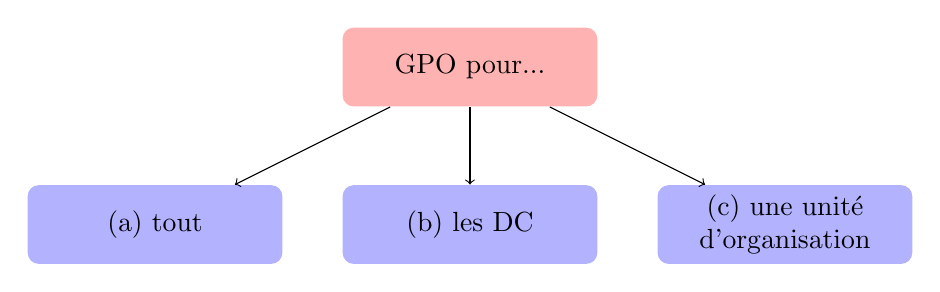
\begin{tikzpicture}
        
        \node (root) [incolore, fill=red!30, draw=none] at (0,0) {GPO pour...};

        \node (a) [incolore, fill=blue!30, draw=none] at (-4,-2) {(a) tout};
        \node (b) [incolore, fill=blue!30, draw=none] at (+0,-2) {(b) les DC};
        \node (c) [incolore, fill=blue!30, draw=none] at (+4,-2) {(c) une unité d'organisation};

        \draw[->] (root) -- (a);
        \draw[->] (root) -- (b);
        \draw[->] (root) -- (c);

    \end{tikzpicture}
\end{center}



\begin{enumerate} \setcounter{enumi}{1}
    \item dans le menu de gauche, clic droit sur:
    \begin{enumerate}
        \item \textit{forest: domaine.local/default domain policy}
        \item \textit{forest: domaine.local/domains/domaine.local/domain controllers/default domain controllers policy}
        \item une \textit{policy} dans l'unité d'organisation (dans \textit{forest: domaine.local/domains/domaine.local/})
        \begin{example}
            Si il n'y a pas encore de \textit{policy} dans l'unité d'organisation:
            \begin{itemize}
                \item clic droit sur l'unité d'organisation
                \item cliquer sur \textit{create a gpo in this domain and link it here}
            \end{itemize}
        \end{example}
    \end{enumerate}
    \item après le clic droit sur la policy, cliquer sur \textit{edit}
\end{enumerate}
\textbf{Remarque}: différence entre \textit{default domain policy} et \textit{default domain controller policy} (= \textit{default DC policy}):
\begin{itemize}
    \item les paramètres configurés dans \textit{default domain policy} s'appliquent à toutes les machines du domaine
    \item les paramètres dans \textit{default domain controller policy}  ne s'appliquent qu'aux serveurs DC du domaine
\end{itemize}





\subsection{Ajouter une GPO \textit{log on locally}}



\begin{enumerate}
    \item ouvrir le \textit{Group Policy Management Editor} (voir section \ref{sec:GPME})
    \item dans le menu de gauche, cliquer sur \textit{computer configuration/policies/windows settings/security settings/local policies/user rights assignment}
    \item doucle-cliquer sur \textit{allow logon locally}
    \item cliquer sur \textit{add user or group}, puis sur \textit{browse}
    \item écrire \textit{Pamela} en bas, puis cliquer sur \textit{check names}, puis sur \textit{ok}
\end{enumerate}





\subsection{Ajouter une GPO pour autoriser/refuser le ping avec le firewall}



\begin{enumerate}
    \item ouvrir le \textit{Group Policy Management Editor} (voir section \ref{sec:GPME})
    \item dans le menu de gauche, clic droit sur \textit{computer configuration/policies/windows settings/security settings/windows defender firewall/inbound rules}, puis cliquer sur \textit{new rule}
    \item sélectionner l'option \textit{predefined}, puis l'option \textit{file and printer sharing}
    \item cliquer sur \textit{next}, puis sélectionner l'option permettant le ping en ipv4
    \item cliquer sur \textit{next}, puis sélectionner l'option \textit{allow the connection}
\end{enumerate}





\subsection{Ajouter une GPO pour changer la page d'accueil de internet explorer (IE)}



\begin{enumerate}
    \item ouvrir le \textit{Group Policy Management Editor} (voir section \ref{sec:GPME})
    \item dans le menu de gauche, cliquer sur \textit{User Configuration/Policies/Administrative Template/Windows Components/Internet Explorer}
    \item clic droit sur \textit{disable changing home page settings}, puis cliquer sur \textit{edit}
    \item choisir l'option \textit{enabled}, et taper l'adresse dans \textit{home page}: http://www.<site>.<wtv>
\end{enumerate}





\subsection{Ajouter un redirecteur conditionnel (dns)}



\begin{enumerate}
    \item taper \textit{dns manager} dans la barre de recherche windows
    \item dans le menu de gauche, faire un clic droit sur \textit{dns/dc1/conditionnal forwarders}
    \item cliquer sur \textit{new conditionnal forwarder}
    \item dans \textit{dns domain}, taper: <site>.<wtv>
    \item dans \textit{ip addresses of the master servers}, taper l'adresse ip du serveur web
\end{enumerate}





\subsection{Ajouter une zone primaire et un enregistrement A (dns)}



Ajouter une zone primaire:
\begin{enumerate}
    \item taper \textit{dns manager} dans la barre de recherche windows
    \item dans le menu de gauche, faire un clic droit sur \textit{dns/dc1/forward lookup zone}, puis cliquer sur \textit{new zone}
\end{enumerate}


Ajouter un enregistrement A:
\begin{enumerate}
    \item taper \textit{dns manager} dans la barre de recherche windows
    \item dans le menu de gauche, faire un clic droit sur \textit{dns/dc1/forward lookup zone/<zone>}
    \item cliquer sur \textit{new host (A or AAAA)}
    \item dans \textit{name}, taper: www
    \item dans \textit{ip address}, taper l'adresse ip du serveur web
\end{enumerate}





\subsection{Activer le rôle DHCP pour l'AD (pendant l'installation du rôle)}



Lors de la configuration post-installation du rôle DHCP, dans \textit{autorization}, sélectionner l'option \textit{use the following user's credentials}, avec \textit{user name} mis en \textit{domaine$\backslash$administrator}.





\subsection{Ajouter une default gateway dans le dhcp}



\begin{enumerate}
    \item ouvrir le dhcp manager
    \item dans le menu de gauche, faire un clic droit sur \textit{dhcp/ms1.domaine14.local/ipv4/scope[<ip>] labo2/scope option}
    \item cliquer sur \textit{configure options}
    \item cliquer sur \textit{003 router}, et ajouter l'adresse ip de la default gateway
\end{enumerate}





\subsection{Forcer l'adoption immédiate des GPO}



\textbf{ATTENTION !} À faire sur toutes les machines, pas uniquement DC.
\begin{enumerate}
    \item ouvrir CMD
    \item taper la commande \texttt{gpupdate /force}
\end{enumerate}





\subsection{Vérifier les GPO dans le \textit{Group Policy Management}}



\begin{enumerate}
    \item taper \textit{gpmc.msc} dans la barre de recherche windows
    \item cliquer sur la stratégie à vérifier
    \item aller dans l'onglet \textit{settings}
    \item vérifier que les GPO sont bien configurées
\end{enumerate}
\textbf{Remarque}: la fenêtre \textit{group policy management} en se rafraîchit pas, il faut la fermer et la rouvrir si nécessaire.















\section{Comment faire le labo 3}





\subsection{Ajouter un disque et l'initialiser}



Dans VirtualBox:
\begin{enumerate}
    \item cliquer sur la VM, puis sur \textit{configuration}, puis sur \textit{Stockage}
    \item dans \textit{unités de stockage}, cliquer sur \textit{ajouter un disque dur}
    \item choisir les options du disque
\end{enumerate}
Dans la VM:
\begin{enumerate}
    \item taper \textit{computer management} dans la barre de recherche windows
    \item dans le menu de gauche, cliquer sur \textit{disk management}
    \item une fenêtre \textit{initialize disk} devrait s'ouvrir, cliquer sur \textit{ok}
\end{enumerate}





\subsection{Créer un volume et un share de type SMB}



Créer un volume:
\begin{enumerate}
    \item taper \textit{server manager} dans la barre de recherche windows
    \item dans le menu de gauche, cliquer sur \textit{file and storage server}, puis sur \textit{disks}
    \item faire un clic droit sur le dernier disque, puis cliquer sur \textit{new volume}
    \item choisir les options du volume et changer la \textit{drive letter} à \textit{F}
\end{enumerate}
Créer un share de type SMB:
\begin{enumerate}
    \item dans la même fenêtre (\textit{server manager}), dans le menu de gauche, cliquer sur \textit{shares}
    \item en haut, à droite de \textit{shares}, cliquer sur \textit{tasks}, puis sur \textit{new share}
    \item dans \textit{share location}, sélectionner le volume \textit{F}
    \item donner le nom \textit{MyShare} dans \textit{share name}
\end{enumerate}
\textbf{Remarque}: si il n'y a pas \textit{shares} dans le menu de gauche de \textit{server manager}, aller dans \textit{computer management} pour créer le share.





\subsection{Ajouter une GPO pour réduire l'intervalle d'actualisation des GPO}



\begin{enumerate}
    \item ouvrir le \textit{Group Policy Management Editor} (voir section \ref{sec:GPME})
    \item dans le menu de gauche, cliquer sur \textit{computer configuration/policies/administrative templates/system/group policy}
    \item double-cliquer sur \textit{set group policy refresh interval for computers}
    \item activer l'option \textit{enabled}, puis configurer l'intervalle d'actualisation, ensuite appuyer sur \textit{apply}
\end{enumerate}





\subsection{Ajouter une GPO pour interdire notepad aux utilisateurs}



\begin{enumerate}
    \item ouvrir le \textit{Group Policy Management Editor} (voir section \ref{sec:GPME})
    \item dans le menu de gauche, cliquer sur \textit{user configuration/policies/administrative templates/system}
    \item double-cliquer sur \textit{don't run specified windows applications}
    \item sélectionner l'option \textit{enabled}
    \item dans \textit{options}, cliquer sur \textit{show}
    \item dans la fenêtre qui vient de s'ouvrir, ajouter les deux valeurs \textit{notepad}, et \textit{notepad.exe}
    \item appuyer sur \textit{ok}, puis \textit{apply}
\end{enumerate}





\subsection{Ajouter une GPO \textit{lock\_taskbar}}



\begin{enumerate}
    \item ouvrir le \textit{Group Policy Management Editor} (voir section \ref{sec:GPME})
    \item dans le menu de gauche, cliquer sur \textit{user configuration/policies/administrative templates/start menu and taskbar}
    \item double-cliquer sur \textit{lock the taskbar}
    \item sélectionner l'option \textit{enabled}, puis cliquer sur \textit{apply}
\end{enumerate}





\subsection{Ajouter un filtre WMI: mémoire libre > 2Go}



Créer un filtre WMI:
\begin{enumerate}
    \item taper \textit{gpmc.msc} dans la barre de recherche windows
    \item dans le menu de gauche, faire un clic droit sur \textit{wmi filter}, puis cliquer sur \textit{new}
    \item changer le nom et la description, puis cliquer sur \textit{add} et taper la query
    \begin{example}
        exemple -- filtre mémoire libre > 2Go: \\
        \texttt{select * from Win32\_OperatingSystem where FreePhysicalMemory > 2150000000}
    \end{example}
\end{enumerate}
Ajouter un filtre WMI à une GPO:
\begin{enumerate}
    \item taper \textit{gpmc.msc} dans la barre de recherche windows
    \item dans le menu de gauche, cliquer sur la GPO pour laquelle il faut ajouter le filtre WMI
    \item à droite, dans \textit{wmi filtering}, sélectionner le filtre WMI à appliquer
\end{enumerate}





\subsection{Ajouter une GPO de déployement d'application}



Base:
\begin{enumerate}
    \item placer le fichier \textit{.msi} de l'application dans le share SMB
    \begin{example}
        \begin{itemize}
            \item ouvrir le \textit{server manager}, cliquer sur \textit{local server}
            \item désactiver les paramètres de \textit{internet explorer enhanced security configuration}
            \item télécharger le fichier \textit{.msi} dans IE, ex: \texttt{https://chromeenterprise.google/browser/download}
        \end{itemize}
    \end{example}
    \item ouvrir le \textit{Group Policy Management Editor} (voir section \ref{sec:GPME})
    \item dans le menu de gauche, faire un clic gauche puis un clic droit sur \textit{computer configuration/policies/software settings/software installation}
    \item cliquer sur \textit{new}, puis sur \textit{package}, ensuite sélectionner le fichier \textit{.msi} placé dans le share SMB
\end{enumerate}
Complément (pas obligatoire) -- installer uniquement sur une machine:
\begin{enumerate}
    \item dans la fenêtre \textit{group policy management}, dans le menu de gauche, cliquer sur la GPO de déployement d'application
    \item à droite, en-dessous de \textit{security filtering}, retirer le groupe des utilisateurs authentifiés
    \item ensuite, cliquer sur \textit{add}, puis sur \textit{object types}, et ajouter les ordinateurs
    \item ensuite, taper le nom de machine, puis cliquer sur \textit{check names}
\end{enumerate}
Après avoir appliqué les GPO sur la machine, il faut la redémarrer pour lancer l'installation.





\subsection{Ajouter un modèle d'administration}



\begin{enumerate}
    \item ouvrir le \textit{Group Policy Management Editor} (voir section \ref{sec:GPME})
    \item dans le menu de gauche, faire un clic droit sur \textit{computer management/administrative templates}
    \item cliquer ensuite sur \textit{add/remove templates}, puis sur \textit{add}
    \item sélectionner le fichier \textit{.adm} qui doit être situé dans le Share SMB
\end{enumerate}





\subsection{Installer le rôle \textit{remote access}}



\begin{enumerate}
    \item ouvrir le \textit{server manager}, en haut à droite, cliquer sur \textit{manage}, puis sur \textit{add roles and features}
    \item dans \textit{server roles}, cliquer sur \textit{remote access}, dans \textit{role services}, cliquer sur \textit{routing}
    \item une fois l'installation terminée, dans le menu de gauche de \textit{server manager}, cliquer sur \textit{remote access}
    \item au centre de la fenêtre, faire un clic droit sur le serveur, puis cliquer sur \textit{remote access management}
    \item dans le menu de gauche, cliquer sur \textit{directaccess and vpn}
    \item ensuite après le chargement, dans le menu de droite, cliquer sur \textit{open rras management}
    \item dans la nouvelle fenêtre, clic droit sur le serveur, puis sur \textit{configure and enable routing and remote access}
    \item dans \textit{configuration}, sélectionner l'option \textit{network address translation (nat)}
\end{enumerate}


\textcolor{red}{\textbf{Attention !}}
\begin{itemize}
    \item Mettre le DNS sur DC1.
    \item Mettre la default gateway sur MS1.
    \item En cas de problème, ouvrir \textit{RRAS management}:
    \begin{enumerate}
        \item dans le menu de gauche, supprimer \textit{ms1/ipv4/nat}
        \item dans le menu de gauche, faire un clic droit sur \textit{ms1/ipv4/general}, puis sur \textit{new routing protocol}
        \item ajouter le \textit{nat}
        \item dans le menu de gauche, faire un clic droit sur \textit{ms1/ipv4/nat}, puis sur \textit{new interface}
        \item ajouter l'interface sur réseau interne en \textit{private interface connected to private network}
        \item ajouter l'interface en réseau externe en \textit{public interface connected to the internet}, \textbf{et} \textit{enable nat on this interface}
    \end{enumerate}
\end{itemize}















\section{Comment faire le labo 4}





\subsection{Créer un dossier invisible et changer les accès}



\begin{enumerate}
    \item Créer le dossier (directement dans le filesystem, pas dans le share).
    \item Pour modifier les accès au dossier, faire un clic droit sur le dossier, cliquer sur \textit{properties}, puis aller dans l'onglet \textit{security}.
    \item Dans le menu de gauche de \textit{server manager}, cliquer sur \textit{file and storage service}, puis sur \textit{shares}.
    \item À droite du menu \textit{shares}, cliquer sur \textit{tasks}, puis sur \textit{new share}.
    \item Dans \textit{share name}, ajouter un \$ à la fin du nom.
\end{enumerate}
\textbf{Remarque}: il faudra taper le \$ dans l'explorateur de fichiers pour accéder au share.






\subsection{Créer un utilisateur itinérant} \label{sec:utilisateuritinerant}



\begin{enumerate}
    \item ouvrir la fenêtre \textit{active directory users and computers}
    \begin{enumerate}
        \item ouvrir le \textit{server manager}
        \item à gauche, cliquer sur \textit{AD DS}
        \item faire un clic droit sur \textit{DC1}, puis cliquer sur \textit{active directory users and computers}
    \end{enumerate}
    \item faire un clic droit sur l'utilisateur, puis cliquer sur \textit{properties}, ensuite sélectionner l'onglet \textit{profile}
    \item dans \textit{profile path}, donner un lien vers le share (ex: \texttt{$\backslash$$\backslash$ms1$\backslash$profiles\$$\backslash$\%username\%})
\end{enumerate}





\subsection{Créer un utilisateur obligatoire}



\begin{enumerate}
    \item créer un utilisateur itinérant (section: \ref{sec:utilisateuritinerant})
    \item se connecter avec l'utilisateur et aller dans le dossier qui contient les dossiers de profils de l'utilisateur
    \item faire un clic droit sur son dossier, puis cliquer sur \textit{properties}
    \item aller dans l'onglet \textit{security}, cliquer sur \textit{edit}, et ajouter l'administrateur du domaine en \textit{full control}
    \item se reconnecter en administrateur du domaine, et aller dans le dossier de l'utilisateur
    \item modifier l'extension du fichier \textit{ntuser.dat}, dans le dossier du profil de l'utilisateur, en \textit{.man}
\end{enumerate}
\textbf{Remarques}:
\begin{itemize}
    \item l'administrateur du domaine doit avoir \textit{full control} sur le dossier de l'utilisateur
    \item pour voir le fichier, il faut activer l’affichage des fichiers cachés
\end{itemize}





\subsection{Vérifier le type d'un profil (itinérant, obligatoire)}



\begin{enumerate}
    \item taper \textit{panneau de configuration} dans la barre de recherche windows
    \item cliquer sur \textit{système et sécurité}, puis sur \textit{système}, puis sur \textit{paramètres système avancés}
    \item en-dessous de \textit{profil des utilisateurs}, cliquer sur \textit{paramètres}
\end{enumerate}





\subsection{Ajouter une GPO pour rediriger les dossiers personnels}



\begin{enumerate}
    \item ouvrir le \textit{Group Policy Management Editor} (voir section \ref{sec:GPME})
    \item dans le menu de gauche, faire un clic droit sur \textit{user configuration/policies/windows settings/folder redirection/documents}
    \item cliquer sur \textit{properties}, dans \textit{setting}, sélectionner \textit{basic}
    \item dans \textit{target folder location}, sélectionner \textit{create a folder for each user under the rooth path}
    \item \textit{root path}, donner un dossier dans le share (ex: \textit{$\backslash$$\backslash$ms1$\backslash$user\_folders})
\end{enumerate}
Modifier le filtre de sécurité:
\begin{enumerate}
    \item dans la fenêtre \textit{group policy management}, cliquer sur la GPO
    \item à droite, enlever \textit{authenticated users}, et ajouter les utilisateurs pour lesquels on veut que la GPO s'applique
    \item aussi ajouter \textit{domain computers}, sinon l'ordinateur ne pourra pas récupérer cette GPO
\end{enumerate}





\subsection{Ajouter une GPO pour interdire toutes les applications dans un dossier}



\begin{enumerate}
    \item ouvrir le \textit{Group Policy Management Editor} (voir section \ref{sec:GPME})
    \item dans le menu de gauche, faire un clic droit sur \textit{computer configuration/policies/windows settings/security settings/software restriction policies}
    \item faire un clic droit sur \textit{additional rule}, puis cliquer sur \textit{new path rule}
    \item cliquer sur \textit{browse}, puis sélectionner le dossier à bannir
\end{enumerate}





\subsection{Ajouter une GPO pour interdire une application avec son hash}



\begin{enumerate}
    \item ouvrir le \textit{Group Policy Management Editor} (voir section \ref{sec:GPME})
    \item dans le menu de gauche, faire un clic droit sur \textit{computer configuration/policies/windows settings/security settings/software restriction policies}
    \item cliquer sur \textit{new software restriction policies}
    \item faire un clic droit sur \textit{additional rule}, puis cliquer sur \textit{new hash rule}
    \item cliquer sur \textit{browse}, puis sélectionner l'application à bannir
\end{enumerate}





\subsection{Joindre le serveur Debian au domaine et permettre aux utilisateurs de s'y logger}



\begin{enumerate}
    \item \texttt{realm join domaine<nb>.local -{}-user=administrator -{}-install='/' -{}-verbose}
    \item \texttt{nano /etc/ssh/sshd\_config}
    \begin{example} \begin{verbatim}
KereberosAuthentification yes
KereberosOrLocalPasswd yes
KereberosTicketCleanup yes
KereberosGetASFToken yes
KereberosUseKuserok yes # pour debian 9, pas debian 10
GSSAPIAuthentification yes
GSSAPICleanupCredentials yes
    \end{verbatim} \end{example}
\end{enumerate}
Vérification:
\begin{enumerate}
    \item \texttt{login pamela@domaine<nb>.local}
    \item \texttt{id}
\end{enumerate}




















\end{document}
